\documentclass{beamer}
%
% Choose how your presentation looks.
%
% For more themes, color themes and font themes, see:
% http://deic.uab.es/~iblanes/beamer_gallery/index_by_theme.html
%
\mode<presentation>
{
  \usetheme{default}      % or try Darmstadt, Madrid, Warsaw, ...
  \usecolortheme{default} % or try albatross, beaver, crane, ...
  \usefonttheme{default}  % or try serif, structurebold, ...
  \setbeamertemplate{navigation symbols}{}
  \setbeamertemplate{caption}[numbered]
} 

\usepackage[english]{babel}
\usepackage[utf8x]{inputenc}
\usepackage{braket}
\usepackage{graphicx}
\usepackage{pgfplots}


\title[Your Short Title]{Accelerated Dynamics in HMC Simulations of Lattice Field
Theory}
\author{Jack Frankland}
\institute{University of Edinburgh}
\date{\today{}}

\begin{document}

\begin{frame}
  \titlepage
\end{frame}

% Uncomment these lines for an automatically generated outline.
%\begin{frame}{Outline}
%  \tableofcontents
%\end{frame}

\section{Introduction}

\begin{frame}{Introduction}

\begin{itemize}
  \item<1-> What are we  doing? 
    \begin{itemize}
        \item Calculating properties of Quantum Mechanical Systems.
    \end{itemize}
  \item<2-> How are we doing it?
    \begin{itemize}
        \item Using MCMC (Markov chain Monte Carlo) methods.
    \end{itemize}
  \item<3-> What results have we got?
  \begin{itemize}
        \item Successfully reproduced harmonic and enharmonic oscillator properties.
    \end{itemize}
  \item<4-> Why are we doing it?
  \begin{itemize}
    \item Can be used for calculations in lattice field theory.
  \end{itemize}
\end{itemize}



\end{frame}

\section{Theory}

\section{Numerics}

\section{Results}

\setbeamercovered{invisible}
\begin{frame}{Results - Harmonic Oscillator Expectation Values}
    \begin{figure}
        \begin{table}
            \begin{tabular}{c | c | c | c }
                Value & Measured & Discrete Theory & Continuum Theory \\
                \hline \hline
                $\braket{x}$   & FILL &  $0$            & $0$           \onslide<2->\\ 
                $\braket{x^2}$ & FILL &  $0.4472135955$ & $\frac{1}{2}$ \onslide<3->\\
                $E_0$          & FILL &  $0.4472135955$ & $\frac{1}{2}$ \onslide<4->\\
                $E_1$          & FILL &  FILL           & $\frac{3}{2}$  
            \end{tabular}
            \caption{Expectation Values for quantum harmonic oscillator with $\mu^2 = 1$, $\text{lattice spacing} = 1$, $\text{lattice size} = 1000$}
        \end{table}
    \end{figure}
\end{frame}

\begin{frame}{Results - Harmonic Oscillator Potential}
    \begin{figure}
    \centering
        \begin{tikzpicture}
            \begin{axis}[
                xlabel= {$x$},
                ylabel= {$V(x)$},
                enlargelimits=true,
                ]
                \addplot[domain=-4:4, samples=100, color=black,]{0.5*x^2};
                \addlegendentry{$V(x)=\frac{\mu^2}{2}x^2$}

            \end{axis}
        \end{tikzpicture}
        \caption{Harmonic Oscillator Potential with $\mu^2 = 1$.}
    \end{figure}
\end{frame}

\begin{frame}{Results - Harmonic Oscillator Wave Function}
    \begin{figure}
    \centering
        \begin{tikzpicture}
            \begin{axis}[
                xlabel= {$x$},
                ylabel= {$\psi{\left(x \right)}$},
                enlargelimits=true,
                ]
                \addplot[color=black,mark=x,]
                    plot [error bars/.cd, y dir = both, y explicit]
                    table[x index=0, y index=1, y error index=2]{DataForPresentation/HarmonicWaveFunction.dat};

            \end{axis}
        \end{tikzpicture}
        \caption{Continuum, discrete and measured wave functions for the harmonic oscillator with $\mu^2 = 1, m = 1, a = 1, L = 1000, d = 0.1, N = 10, \text{configurations} = 100000, \text{burn period} = 1000$.}
    \end{figure}
\end{frame}

\begin{frame}{Results - Harmonic Oscillator Typical Trajectory}
    \begin{figure}
    \centering
        \begin{tikzpicture}
            \begin{axis}[
                xlabel= {Lattice Site},
                ylabel= {$x$},
                enlargelimits=true,
                ]
                \addplot[color=black,mark=x,]
                    table[x index=0, y index=1]{DataForPresentation/HarmonicTypicalTrajectory.dat};

            \end{axis}
        \end{tikzpicture}
        \caption{Typical configuration for the harmonic oscillator with $\mu^2 = 1, m = 1, a = 1, L = 1000, d = 0.1, N = 10, \text{configurations} = 100000, \text{burn period} = 1000$.}
    \end{figure}
\end{frame}

\begin{frame}{Results - Anharmonic Oscillator Potential}
    \begin{figure}
    \centering
        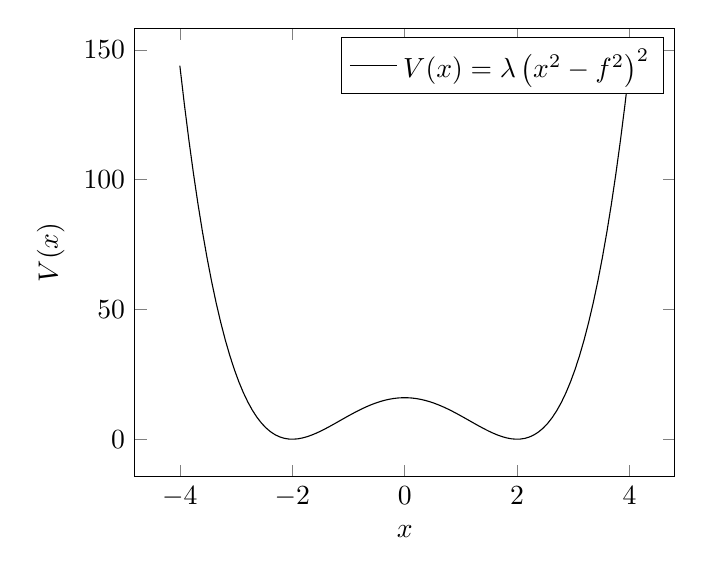
\begin{tikzpicture}
            \begin{axis}[
                xlabel= {$x$},
                ylabel= {$V(x)$},
                enlargelimits=true,
                ]
                \addplot[domain=-4:4, samples=100, color=black,]{x^4-8*x^2+16};
                \addlegendentry{$V(x)=\lambda\left(x^2-f^2\right)^2$}

            \end{axis}
        \end{tikzpicture}
        \caption{Harmonic Oscillator Potential with $\mu^2 = 1$.}
    \end{figure}
\end{frame}

\begin{frame}{Results - Anharmonic Oscillator Expectation Values}
    \begin{figure}
        \begin{table}
            \begin{tabular}{c | c | c | c }
                Value & Measured & Reference Values \\
                \hline \hline
                $\braket{x}$   & FILL &  $FILL$             \onslide<2->\\ 
                $\braket{x^2}$ & FILL &  $FILL$  \onslide<3->\\
                $E_0$          & FILL &  $FILL$  \onslide<4->\\
                $E_1$          & FILL &  $FILL$             
            \end{tabular}
            \caption{Expectation Values for quantum anharmonic oscillator with $\mu^2 = 1$, $\text{lattice spacing} = 1$, $\text{lattice size} = 1000$}
        \end{table}
    \end{figure}
\end{frame}

\begin{frame}{Results - Anharmonic Oscillator Wave Function}
    \begin{figure}
    \centering
        \begin{tikzpicture}
            \begin{axis}[
                xlabel= {$x$},
                ylabel= {$\psi{\left(x \right)}$},
                enlargelimits=true,
                ]
                \addplot[color=black,mark=x,]
                    plot [error bars/.cd, y dir = both, y explicit]
                    table[x index=0, y index=1, y error index=2]{DataForPresentation/AnharmonicWaveFunction.dat};

            \end{axis}
        \end{tikzpicture}
        \caption{Measured wave function for the harmonic oscillator with $\lambda = 1, f^2=4 m = 1, a = 1, L = 1000, d = 0.01, N = 100, \text{configurations} = 100000, \text{burn period} = 1000$.}
    \end{figure}
\end{frame}

\begin{frame}{Results - Anharmonic Oscillator Typical Trajectory}
    \begin{figure}
    \centering
        \begin{tikzpicture}
            \begin{axis}[
                xlabel= {Lattice Site},
                ylabel= {$x$},
                enlargelimits=true,
                ]
                \addplot[color=black,mark=x,]
                    table[x index=0, y index=1]{DataForPresentation/AnharmonicTypicalTrajectory.dat};

            \end{axis}
        \end{tikzpicture}
        \caption{Typical configuration for the anharmonic oscillator with $\lambda = 1, f^2 = 4, m = 1, a = 1, L = 1000, d = 0.01, N = 100, \text{configurations} = 100000, \text{burn period} = 1000$.}
    \end{figure}
\end{frame}

\begin{frame}{Results - A Deeper Anharmonic Oscillator Potential}
    \begin{figure}
    \centering
        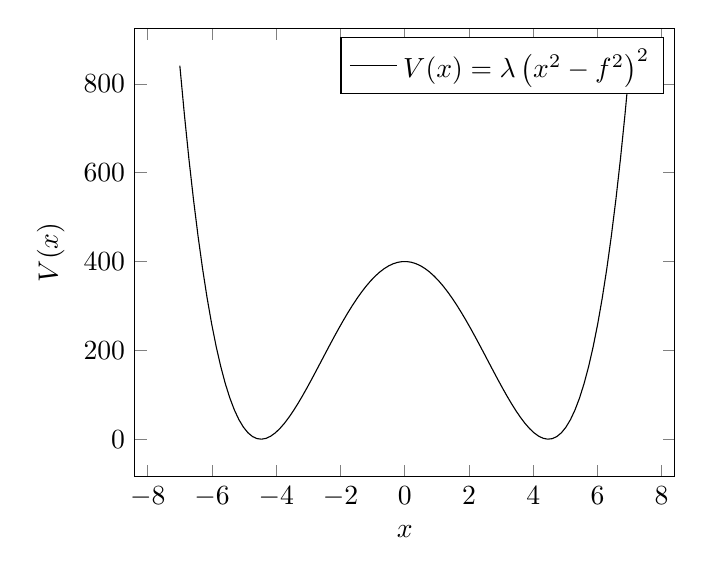
\begin{tikzpicture}
            \begin{axis}[
                xlabel= {$x$},
                ylabel= {$V(x)$},
                enlargelimits=true,
                ]
                \addplot[domain=-7:7, samples=100, color=black,]{x^4-40*x^2+400};
                \addlegendentry{$V(x)=\lambda\left(x^2-f^2\right)^2$}

            \end{axis}
        \end{tikzpicture}
        \caption{Anharmonic Oscillator Potential with $\lambda = 1$, $f^2 = 20$}
    \end{figure}
\end{frame}

\begin{frame}{Results - A Deeper Anharmonic Oscillator Wave Function}
    \begin{figure}
    \centering
        \begin{tikzpicture}
            \begin{axis}[
                xlabel= {$x$},
                ylabel= {$\psi{\left(x \right)}$},
                enlargelimits=true,
                ]
                \addplot[color=black,mark=x,]
                    plot [error bars/.cd, y dir = both, y explicit]
                    table[x index=0, y index=1, y error index=2]{DataForPresentation/AnharmonicWaveFunction.dat};

            \end{axis}
        \end{tikzpicture}
        \caption{Measured wave function for the harmonic oscillator with $\lambda = 1, f^2=4 m = 1, a = 1, L = 1000, d = 0.01, N = 100, \text{configurations} = 100000, \text{burn period} = 1000$.}
    \end{figure}
\end{frame}

\begin{frame}{Results - A Deeper Anharmonic Oscillator Typical Trajectory}
    \begin{figure}
    \centering
        \begin{tikzpicture}
            \begin{axis}[
                xlabel= {Lattice Site},
                ylabel= {$x$},
                enlargelimits=true,
                ]
                \addplot[color=black,mark=x,]
                    table[x index=0, y index=1]{DataForPresentation/AnharmonicTypicalTrajectory.dat};

            \end{axis}
        \end{tikzpicture}
        \caption{Typical configuration for the anharmonic oscillator with $\lambda = 1, f^2 = 4, m = 1, a = 1, L = 1000, d = 0.01, N = 100, \text{configurations} = 100000, \text{burn period} = 1000$.}
    \end{figure}
\end{frame}






\section{Conclusion}
\begin{frame}{Conclusion}
\begin{itemize}
  \item<1-> Did it work? 
    \begin{itemize}
        \item Successfully reproduced known values using HMC method.
    \end{itemize}
  \item<2-> What next?
    \begin{itemize}
        \item Introduce ``tempering'' into the dynamics to sample from isolated modes.
    \end{itemize}
  \item<3-> Applications of tempering?
  \begin{itemize}
        \item Potentially applicable to lattice field theory where computation time is far more costly.
    \end{itemize}
\end{itemize}
\end{frame}
\end{document}
